\section{Componente Servidora}\label{sec33}

A \gls{api-web} é a interface exposta pela componente servidora baseada em \acrshort{http} \cite{RFC7231:http}. A \gls{api-web} disponibiliza informação e funcionalidades fornecidas pelo sistema Smart Stocks, através de \textit{endpoints} públicos e privados.

A decisão de utilizar a \textit{framework} \textit{Spring Boot} para implementar o servidor deve-se ao facto de ser uma ferramenta \gls{open-source}, capaz de criar rapidamente aplicações com auto-configuração, através de anotações. Outra vantagem é a integração com tecnologias de persistência de dados, como a \acrfull{jpa}. Por fim, por questões de conhecimento e de experiência anterior com esta \textit{framework}.

O servidor processa pedidos \acrshort{http} por parte das aplicações cliente. Antes dos pedidos serem processados são sujeitos ao controlo de segurança, que é responsável por validar as credenciais presentes no  \textit{header} \acrshort{http} \textit{Authorization}. 

\begin{figure}[H]
    \hspace*{-1,3cm}
	\centering
	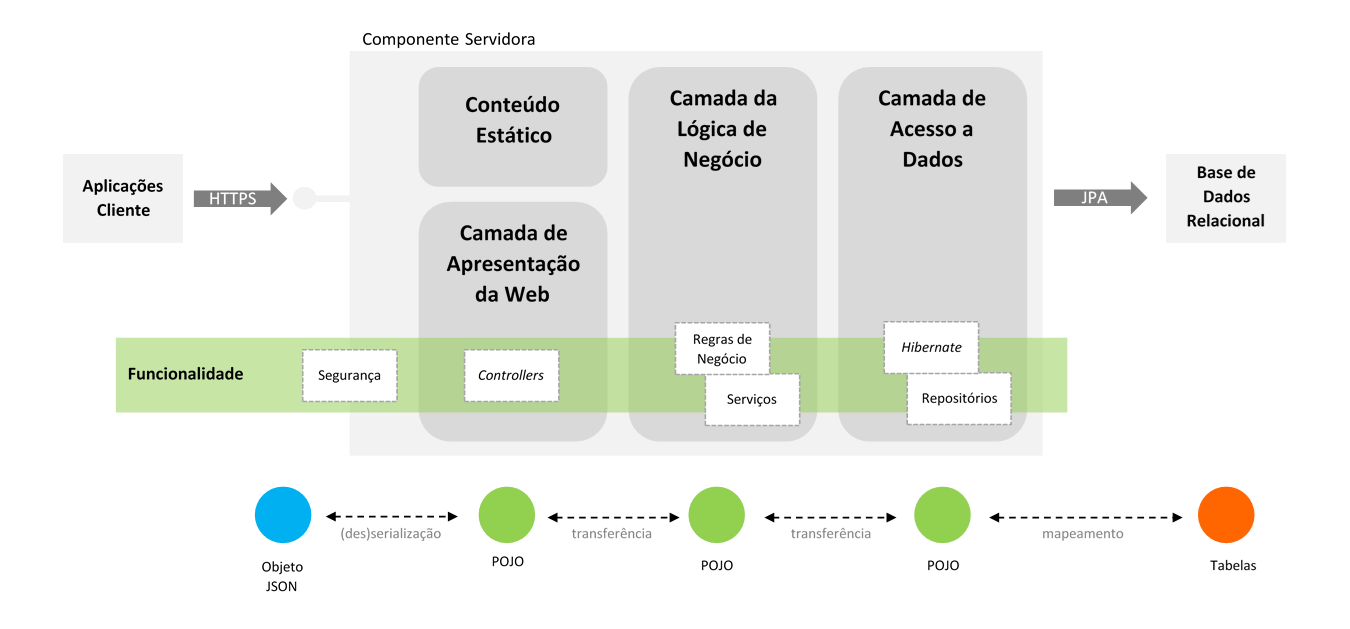
\includegraphics[width=18cm, scale=1]{img/server.png}
	\caption{Arquitetura da Componente Servidora}
	\label{server-architecture}
\end{figure}

Como se pode observar na Figura \ref{server-architecture} o servidor é constituído por 4 blocos, que se enumeram de seguida. O Conteúdo Estático está encarregue de providenciar os dados inalteráveis, i.e., que são independentes do pedido, como por exemplo, as mensagens de erro e a página inicial, que contém informação relativa à API e os links para os recursos. A Camada de Apresentação da Web é responsável por processar os pedidos aos diferentes \textit{endpoints} e produzir uma resposta. É na Camada da Lógica de Negócio que são verificadas as regras de negócio a aplicar aos pedidos. Nesta camada constitui assim o aglomerado de serviços que acedem aos respetivos repositórios. Por último, a Camada de Acesso a Dados garante o acesso à base de dados relacional. Com uma implementação de \acrshort{jpa}, através de repositórios específicos a cada entidade.

À receção de um pedido no servidor, os objetos \acrfull{json} são desserializados em \textit{InputModel} (representações gerais do objeto), de seguida são transformados em objetos \acrfull{pojo}, os quais fluem ao longo das camadas descendentes de todo o processo. No final, estes objetos são mapeados em tuplos das tabelas presentes na base de dados. Já no extremo oposto do processamento da resposta ascendente, o objeto POJO é transformado em \textit{OutputModel} (representações específicas do objeto segundo \textit{hypermedia} utilizada) para assim ser serializado num objeto \acrshort{json}, de forma a poder retornar a resposta ao cliente.


\subsubsection{Internacionalização}

A API desenvolvida ao longo do projeto tem suporte multi-línguas. Esta funcionalidade é importante pois permite que as aplicações cliente usufruam de mensagens de erro na língua em que for feito o pedido. 

Para suportar a funcionalidade de internacionalização faz-se uso do \textit{header} \acrshort{http} \textit{Accept-Language}. No entanto, poderia ser utilizado um parâmetro na \textit{query string} para identificar a linguagem pretendida. Porém, segundo a Google \cite{LeverageBrowserCaching:google} não se deve usar \textit{query string} pelo simples facto de que alguns intermediários, por exemplo, sistemas de \textit{cache}, não observam a \textit{query string}, não distinguindo assim os recursos. Uma outra desvantagem em usar um parâmetro na \textit{query string} deve-se a esta não ser \textit{standard}. 

Os idiomas disponibilizados são inglês e português, sendo a linguagem inglês a linguagem por omissão. Para aceder às mensagens, o \textit{Spring Boot} disponibiliza uma implementação da interface \textit{MessageSource}, que contém um método para aceder a uma mensagem numa determinada língua.


\subsubsection{\textit{Logging}}

Sendo uma grande parte do tempo dos programadores gasta na monitorização, resolução de problemas e \textit{debugging} é interessante manter ficheiros de \acrfull{log} na manutenção de uma aplicação.

Com a criação de registos sobre a execução das aplicações, a tarefa de inspecionar o software e atuar adequadamente perante erros é facilitada. Visto que, se consegue perceber quais os pedidos e respostas que foram efetuados, de maneira a replicar e resolver eventuais falhas.

Para cada pedido \acrshort{http} recebido na API, é feito \textit{logging} do \acrfull{ip} e do porto remoto, do método \acrshort{http}, do \textit{\acrfull{uri}} do pedido \acrshort{http} e de todos os \textit{headers} \acrshort{http} à exceção do \textit{header} \acrshort{http} \textit{Authorization}. Já na resposta do pedido é feito o registo do \textit{status code}, assim como todos os \textit{headers}. 

\subsubsection{Documentação}

É de extrema importância ter a API documentada, tal permite que futuros clientes possam empregar-se dessa mesma documentação e interagir com a API.

O desenvolvimento da documentação foi executado com o auxílio do Swagger \cite{Swagger:api}. Com esta biblioteca especificam-se os diferentes \textit{endpoints} existentes e é gerada uma página HTML com a coletânea de \textit{endpoints}, a partir dos quais é possível realizar testes. Para cada \textit{endpoint} apresentam-se os possíveis \textit{status codes} \acrshort{http} a comporem a resposta, bem como, um exemplo de uma representação de um recurso em caso de sucesso. Permite-se ainda, autenticar os pedidos que assim o exigem. Ao testar um \textit{endpoint}, é retornada a resposta e os \textit{headers} \acrshort{http} da mesma. Para os pedidos que contêm corpo no pedido \acrshort{http} é concedido um exemplo deste e permite-se a inserção de valores para o \textit{endpoint} a ser testado. No caso dos pedidos que necessitam de enviar valores na \textit{path} do \textit{endpoint} é disponibilizada uma caixa de texto para inserir o valor variável. 

A documentação da API permite testar os \textit{endpoints} individualmente e está presente em \textbf{/v1/documentation/swagger-ui.html}


%
% Segurança
%
\subsection{Segurança}\label{subsec334}

Sendo o Smart Stocks um sistema de gestão de stocks domésticos é importante assegurar a confidencialidade e a segurança dos dados de cada casa. Como tal, o acesso a recursos ou a manipulação dos mesmos só pode suceder de forma autenticada e autorizada. Foram pensadas várias soluções para a segurança do sistema.

Uma primeira solução foi usar um servidor de autorização já implementado. Para tal ponderou-se fazer-se uso do projeto \textit{MITREid Connect} \cite{mitreidconnect:impl}, por questões de familiaridade. Este projeto pode ser usado como \textit{IdProvider}, segundo o protocolo \textit{OpenId Connect} \cite{OpenIDConnect:introduction}, ou como servidor de autorização, segundo o protocolo \textit{OAuth2.0} \cite{OAuth20:introduction}. Esta opção foi rejeitada uma vez que este projeto não contém uma página de registo para novos utilizadores. Realizou-se uma pesquisa de implementações de servidores de autorização disponíveis para \textit{Java}. Os projetos encontrados foram o \textit{APIs} \cite{OAuthApis:impl} e \textit{Tokens} \cite{tokens:impl}. Contudo, estes também não disponibilizam uma página de registo para novos utilizadores, logo a ideia de usar um projeto de um servidor de autorização foi igualmente descartada . 

A outra solução passava por desenvolver um servidor de autorização. No entanto, desenvolver um servidor de autorização é complexo, pelo que existem diversos aspetos de segurança importantes para a realização deste tipo de servidores. Com auxílio do \textit{Spring Security} este processo torna-se mais simples. Porém, ainda existe um aspeto fundamental, que é assinar os \textit{tokens}. Para estes seria útil empregar \textit{Json Web Token} (JWT) \cite{JSONWebT8:introduction}, permitindo revogá-los. Todavia, implementar estes servidores é moroso e pouco trivial. 

A solução adotada passa por utilizar outro mecanismo mais básico, o \textit{Basic Scheme Authentication} \cite{RFC7617:basicSheme}. Ao assumir a utilização do protocolo \acrfull{https} \cite{RFC2660:https} (TLS) \cite{RFC5246T88:tls} cria-se um canal com comunicação segura que permite assim utilizar \textit{Basic Authentication}. Com auxílio do \textit{Spring Security} a implementação é facilitada e tem suporte a papéis (\textit{roles}). No sistema Smart Stocks existem dois papéis, o papel \textit{USER} e o papel \textit{ADMIN}, sendo este último a ser utilizado pela aplicação \textit{back-office} a desenvolver no futuro. Os utilizadores registados pelo sistema, ficam automaticamente com o papel \textit{USER}. O papel \textit{USER}, neste momento, tem acesso a todas as funcionalidades implementadas que necessitam de autenticação.
De momento, o papel \textit{ADMIN} não tem qualquer privilégio, mas no futuro este terá funcionalidades de administração do sistema Smart Stocks. Esta foi a solução implementada, no entanto é um dos aspetos a melhorar futuramente.

\subsubsection{\acrlong{cors}}

Ao desenvolver uma API que possa ser acessível através de pedidos que tenham um endereço diferente do endereço da API, por exemplo, feitos por código \textit{JavaScript} a ser executado num \textit{browser} usando AJAX \cite{Ajax:mozilla}, é preciso configurar a API para responder de forma a que o resultado possa ser visível no \textit{browser}. O objeto \textit{XMLHttpRequest} \cite{XMLHttp:online} usa a política de \textit{same-origin}. A especificação \acrfull{w3c} para \acrfull{cors} \cite{CrossOrigin:resource}, permite que os resultados se tornem visíveis, evitando assim a política de segurança imposta pelos \textit{browsers}. Assim deu-se permissão para todos os endereços e todos os \textit{headers} \acrshort{http}, de forma a que os utilizadores da API possam aceder livremente a esta através do \textit{browser}. Com auxílio do \textit{Spring Security} a configuração é realizada como se mostra no Exemplo 1.

\newcounter{ExampleCounter2}
\stepcounter{ExampleCounter2}
\hspace{-1.25cm}
\resizebox{0pt}{0pt}{0pt}{
\noindent\fbox{
	\parbox{\textwidth+5mm}{
		\textbf{Exemplo \arabic{ExampleCounter2}}\\
		\lstinputlisting[language=Java, basicstyle=\small]{code/webSecurityConfig.java}
	}
	}
}\\[0.25cm]


\subsubsection{Armazenamento de \textit{Passwords}}

É considerada má prática o armazenamento de informação sensível, tal como, as de \textit{passwords} em claro na base de dados, então estas devem ser encriptadas antes de serem armazenadas.

Para a encriptação é feito o \textit{hash} da palavra-chave adicionando um valor aleatório. A este valor aleatório dá-se o nome de \textit{salt}. Com o uso de \textit{salt} previne-se que palavras-chave iguais sejam armazenadas na base de dados com valores iguais. 

Caso alguém consiga aceder à base de dados não consegue descobrir a palavra-passe de um determinado utilizador, isto é garantido encriptando a palavra-chave. Para encriptar as palavras-chave usou-se uma implementação do algoritmo \textit{BCrypt} \cite{BCrypt:spring-security} fornecido pelo \textit{Spring Security}. Outras opções passariam por usar o algoritmo \textit{MD5}, ou \textit{SHA}, mas estes estão \textit{deprecated} por serem algoritmos com fraca classificação \cite{DeprecatedAlgorithms:online}. Na implementação do \textit{Spring Security} o \textit{salt} é gerado internamente, ficando concatenado com a \textit{password} cifrada.

%
% Controllers
%
\subsection{\textit{Controllers}}\label{subsec333}

Os \textit{controllers} identificam os pedidos e direciona-os para os serviços adequados ao seu processamento, retornando no final a resposta apropriada. Os formatos de resposta utilizam \textit{hypermedia} \cite{APIBestP87:hypermedia}, e são de um de três tipos: \textit{Json Home} \cite{draftnot72:jsonHome} utilizado para representar a página inicial da \gls{api-web}, \textit{Siren} \cite{kevinswiber:siren} representa respostas em que o \textit{status code} \acrshort{http} representa sucesso e \textit{Problem Details} \cite{RFC7807:problemDetails} para representar respostas em que o \textit{status code} \acrshort{http} representa erro.

A escolha do uso de \textit{hypermedia} apoia-se em questões evolutivas da API em termos de hiperligações, ou seja, caso os \textit{endpoints} dos recursos sejam alterados a aplicação cliente não sofre alterações.

Hoje em dia é comum encontrar uma API que se classifique no nível dois, segundo o modelo de maturidade definido pelo Leonard Richardson \cite{RichardsonMaturityModel:martinFowler}. Pertencer ao nível dois significa que é retornada informação relativa ao recurso pedido, não existindo nenhuma meta informação associada ao recurso. Logo, para se conhecer as operações disponíveis e permitidas sobre esse recurso, ou ter conhecimento dos links para os recursos relacionados com o recurso retornado, é indispensável a consulta da documentação da API. 

Já no nível três, do modelo supramencionado, estas informações são retornadas em conjunto com a representação do recurso, estando presente a representação da entidade e meta informação associada ao recurso retornado. Uma outra vantagem do nível três é que as aplicações cliente apenas contém um link \textit{hardcoded}, sendo este o \acrfull{url} para a página inicial, denominado link base. Pelo que passa a ser responsabilidade da API embeber os links nas representações. Assim, se algum link sofrer alterações, nenhuma aplicação cliente fica comprometida.

Existem desvantagens no nível três comparado com o nível dois. Por exemplo, as mensagens de resposta \acrshort{http} serem de maior dimensão, usando uma maior largura de banda. Uma outra desvantagem é as aplicações cliente necessitarem de mapear as representações recebidas pela API e fornecerem uma \textit{user interface} com base na representação recebida, o que aumenta o grau de complexidade no desenvolvimento.

Chegou-se à conclusão que usar controlos com \textit{hypermedia} seria mais vantajoso para o projeto, pois as regras de negócio são definidas pela API e estão embebidas nas representações em \textit{hypermedia}, ver Exemplo 2.\\

\stepcounter{ExampleCounter2}
\noindent\fbox{
	\parbox{\textwidth}{
		\textbf{Exemplo \arabic{ExampleCounter2}}\\	
		
		Tomando como caso as listas do sistema Smart Stocks, existem dois tipos de listas: Listas de Utilizador e Listas de Sistema. As Listas de Utilizador podem ser alteradas tanto pelo utilizador que as criou como pelos utilizadores com os quais a lista foi partilhada. Já as Listas de Sistema são inalteráveis pelos utilizadores. Ora, na representação das listas que um utilizador pode consultar tanto constam Listas de Utilizador como de Sistema. Assim consoante a entidade que se está a representar pode ou não existir a ação de atualizar a lista, conforme se a lista é de Utilizador ou não. Com o uso de \textit{hypermedia} esta regra de negócio é diretamente aplicada na representação da resposta e desde que esta seja corretamente utilizada evita a falha de pedidos, visto que estes não são permitidos. Ver exemplo de resposta no Anexo \ref{seca21}, que representa as listas a que um utilizador tem acesso, no formato \acrshort{json} e utilizando \textit{hypermedia} \textit{Siren}.
	}
}

\subsubsection{Formato dos Erros}
De forma a uniformizar os erros expostos pela API, utilizou-se \textit{hypermedia} \textit{Problem Details}. Esta \textit{hypermedia} permite dar ao utilizador mais informação sobre o erro e como resolve-lo caso seja um erro de cliente. Todos os pedidos realizados à API em que ocorra um erro, é retornada uma representação no formato \textit{Problem Details}.


%
% Lógica de Negócio
%
\subsection{Lógica de Negócio}\label{subsec332}

É fundamental fazer cumprir as regras, restrições e toda a lógica da gestão dos dados para o correto funcionamento do sistema. Assim,  este controlo foi depositado na \acrfull{bll} e também no modelo desenvolvido. Esta decisão permite, não só, concentrar a gestão dos dados, como também, controlar numa camada intermédia os dados a obter, atualizar, remover ou inserir, antes de realizar o acesso/escrita dos mesmos. O que estabelece um conjunto de operações disponíveis e coordena a resposta do aplicativo em cada operação.

Cada serviço estabelece um conjunto de operações disponíveis, conforme a definição de Randy Stafford \cite{PofEAASe2:serviceLayer}. Desta maneira, consegue-se isolar as diversas operações referentes a cada entidade. 

Para a implementação desta camada criaram-se serviços associados a um ou mais \textit{repositories}. Estes expõem funcionalidades e aplicam as regras de negócio necessárias.

%
% Acesso a Dados
%
\subsection{Acesso a Dados}\label{subsec331}

Uma forma de abstrair a \acrshort{bll} do acesso aos dados foi através da definição da \acrshort{dal}, separando as regras de negócio do acesso aos dados.

São várias as formas de realizar o acesso à base de dados, sendo uma delas com a utilização do \acrshort{jdbc} \textit{driver}. Este expõe uma série de interfaces para realizar o acesso, como o \textit{PreparedStatment}, o \textit{ResultSet}, o \textit{CallableStatment}, entre outras. Primeiramente, pensou-se desenvolver o acesso à base de dados através destas interfaces, tendo o programador de se preocupar com a escrita das \textit{queries}, os contextos, o mapeamento do resultado das \textit{queries} em classes \acrshort{pojo}, as transações, a implementação dos padrões de \textit{lazy-loading}, de \textit{repository} e de \textit{unit of work}. Por contexto entendem-se as ligações estabelecidas e a manutenção destas através de um \textit{pool} de ligações. Desenvolver um sistema \acrfull{orm} não é simples e toma algum tempo. Não é âmbito do projeto desenvolver este sistema. 

Uma solução alternativa seria usar \acrfull{jdbctemplate}. Esta biblioteca fornece uma abstração maior sobre a gestão de ligações, não tendo o programador de se preocupar com isso. A desvantagem desta solução seria a escrita de \textit{queries}, o mapeamento dos resultados em classes \acrshort{pojo} e a implementação dos padrões descritos anteriormente. É um contra pois seria código repetitivo, visto que para cada entidade seria necessário escrever \textit{queries} e mapear os resultados em classes \acrshort{pojo} para obter os dados dessa tabela, ou só pelo identificador da entidade, para inserir uma entidade, para atualizar ou apagar. No fundo, garantir as operações \acrfull{crud}, entre outras. 

A solução encontrada foi usar a \acrfull{jpa} \cite{javaee6:jpa}. Esta API permite uma maior abstração quando comparada com \acrshort{jdbctemplate}, devido a não ser requerida a escrita de \textit{queries} nem o mapeamento em classes \textit{Java}, e esta já implementar os padrões mencionados anteriormente. Para ter acesso às operações \acrshort{crud} é necessário criar uma interface, que estenda de uma interface do \acrshort{jpa}. Assim, simplifca-se a implementação das operações básicas. Caso sejam precisas outras operações, é possível declarar métodos nessa interface com nomes específicos do \acrshort{jpa}, para este gerar as \textit{queries} automaticamente, como se mostra no Exemplo 3.\\

\stepcounter{ExampleCounter2}
\hspace{-1.25cm}
\resizebox{0pt}{0pt}{0pt}{
\noindent\fbox{
	\parbox{\textwidth+5mm}{
		\textbf{Exemplo \arabic{ExampleCounter2}}\\
		\lstinputlisting[language=Java, basicstyle=\small]{code/listrepository.java}
		
	}
	}
}\\[0.25cm]


Cada entidade presente na \acrshort{bd} é mapeada numa classe em Java, que representa o modelo de domínio da mesma. Esta classe tem várias anotações da \acrshort{jpa} para referir a \acrlong{cp}, \acrlong{ce}, associações entre entidades, etc. Em conjunto estas classes \textit{Java} formam o modelo utilizado entre as camadas internas do lado do servidor. 
Criaram-se vários \textit{repositories} e cada um encontra-se associado a uma entidade.
A JPA é a especificação, para a implementação foi usado \textit{Hibernate} \cite{Hibernate:online}.